%!TEX root=../mythesis.tex
% Chapter Template

\chapter{Toward Automated Verification of Smart Contract Fairness} % Main chapter title
\chaptermark{FairCon: Toward Automated Verification of Smart Contract Fairness}  % replace the chapter name with its abbreviated form
\label{ch:faircon} 
% Change X to a consecutive number; for referencing this chapter elsewhere, use \ref{ChapterX}

\section{Introduction}\label{Sec_Introduction}
The blockchain technology has been developed rapidly in recent years, since the introduction of
Bitcoin~\cite{nakamoto2008bitcoin} by Nakamoto in 2008.
The distributed and tamper-resistant nature of blockchain has made it the perfect platform for
hosting smart contracts.
%Nowadays, blockchain technology has been widely applied to support many critical complicated
%systems by resorting to Turing-complete smart contract, thus there are a lot of booming
%applications beyond cryptocurrencies, which have not yet to be studied very well.
Smart contracts are computer programs running atop blockchain platforms to manage large sums of
money, carry out transactions of assets, and govern the transfer of digital rights between multiple
parties.
Ethereum~\cite{Ethereum} and EOS~\cite{EOS} are among the most popular blockchain platforms which
support smart contracts and have them applied in many areas.
%Among those platforms, Ethereum is considered one of the most promising where millions of smart
%contracts are running on.
%These smart contracts have shown their enormous capability to apply to diverse fields such as
%electronic auction and computer games, where centralized software platforms have not worked very
%well.
%It also has its unique advantage beyond past technology, especially for some other unexpected
%domains such as the token economy.
As of February 2020, there are over one million smart contracts deployed on Ethereum, which is a 100
fold increase since just two years ago.
These smart contracts have enabled about 2.7K decentralized applications (DApps)~\cite{dapp-stats}
serving 20K daily users on finance, health, governance, gambling, games, etc.
%As we know, in 2019, Moscow adopted smart contract technology in its parliament election
%\cite{election_attacks}.
%However, according to Gaudry reports \cite{gaudry2019breaking}, we know
%that this voting system is not perfect since it is said to be at the risk of encryption leakage.
%We also know that for EOS platforms, attacks to the game have caused faithful players suffering a
%lot, such as Dice, EOS attacks~\cite{EOS_attacks}.
%For the Ethereum platform, the DAO attack~\cite{DAO_attacks} is the most famous security event
%which brings the loss of \$60,000,000 worth, where the attacker exploited the reentrancy
%vulnerability underlying the DAO contract. T
%he smart contract, as a booming technology, is inclined to high chance of being attacked because
%of its immaturity in its characteristics and poor development quality by non-expert developers.

%Therefore with the increasing impact of security events in the smart contract, there are a
%considerable number of researches focus on these security problems. Oyente
%\cite{oyente,luu2016making} deserved high acknowledgment to first present a wide existence of some
%of the mentioned vulnerabilities in the smart contract on a large scale. Atzei et al.
%\cite{atzei2016survey} surveyed and analyzed large amounts of existing attack reports to offer a
%relatively comprehensive taxonomy of vulnerabilities based on different occurring contexts and
%characteristics. At the same time, some researches focus on the detection of malicious smart
%contracts \cite{bhargavan2016formal, grishchenko2018semantic, hirai2016formal,
%hildenbrandt2017kevm, park2018formal}. However, all of them have not considered the properties of
%smart contract beyond the security, which is the fairness property of smart
%contract.

%\begin{comment}
%\yi{This paragraph seems not so directly related. maybe put it in related work. better to focus on
%fairness in the intro: what are the different fairness considerations/properties?}
%Therefore with the increasing impact of security events in smart contract, there is a considerable
%number of researches focus on these security problems, which we can divide into two perspectives.
%One is to migrate traditional program security domain knowledge to the smart
%contract.
%Survey have presented possible bug types in smart contract including common integer overflow, owing
%to which Meitu Coin had been ruined, exception disorder that in essence seems likely to resemble
%exception handling in Java and other programming language. Lots of tools have been created to
%explore these bugs or to avoid these vulnerabilities. Among of which, Oyente
%\cite{oyente,luu2016making} deserved high acknowledgment to first present widely existence of some
%of the mentioned vulnerabilities in smart contract at large scale. The other one could be the
%research coupled with the application domain of
%smart contract. Of the different application domains, ERC token has been studied by many researches.
%[]  Token specification, [] Token event order consistency, [] token behaviors. However, all of
%them have not considered the properties of the smart contract after the security guaranteed, which
%is we focus on the
%fairness properties of the smart contract.
%\end{comment}

The security of smart contracts has been at the center of attention, ever since their adoption in
the management of massive monetary transactions.
One of the most notorious cases is the DAO attack~\cite{DAO_attacks} on Ethereum, which resulted in
a loss of \$60 million worth, due to the \emph{reentrancy vulnerability} being exploited by
malicious attackers.
Several gambling games on EOS, including \texttt{EOS.WIN} and \texttt{EOSPlay}, were recently
hacked using a technique called the \emph{transaction congestion attack}~\cite{EOS_attacks} and led
to significant asset loss.
What these incidents share in common is that certain security vulnerabilities neglected during
contract development are exploited by malicious parties, causing a loss for the contract owners
(and possibly other honest participants).
These vulnerabilities are programming errors, indicating a mismatch between the contract
developers' expectations and how the contract code actually works.
They are easy to detect once the vulnerability patterns are recognized.
In fact, much research has been dedicated to preventing, discovering, and mitigating such attacks.

In contrast, the \emph{fairness} issues of smart contracts have not yet attracted much attention.
A smart contract is unfair to certain participants if there is a mismatch between the participants'
expectations and the actual implementation of the game rules.
It is possible that a malicious party may gain an advantage over others through the exploitation of
security vulnerabilities, e.g., examining other participants' actions in a sealed game.
In this paper, we would like to focus more on the fairness issues introduced by the logical design
of the contracts instead, which are orthogonal to the security issues.
For example, smart contracts may well be advertised as ``social games'' with a promised 20\% return
for any investment, but turn out to be ``Ponzi schemes''~\cite{BARTOLETTI2020259}.
In this case, the possibility that the game may eventually slow down and never pay back is
intentionally left out.
Similarly, many auction DApps claim to be safe and fair, yet it is still possible for bidders to
collude among themselves or with the auctioneer to make a profit at the expenses of the
others~\cite{wu2018cream}.
The fairness issues mostly reside in contract logic: some of them are unfair by design, while the
rest are careless mistakes.
This makes the detection of such issues particularly challenging, because every case can be
different and there is no hope in identifying predefined patterns.
Since it is often not the contract creators' interest at risk (or even worse when they gain at the
expenses of participants), there is little incentive for them to allocate resources in ensuring the
fairness of their contracts.
On the other hand, it is rather difficult, for inexperienced users, to tell whether a contract works
as advertised, even with the source code available.

%The fairness problem exists even though security of smart contract are assured.
%Specifically, mechanism design is to study how to allocate resource to different participants.
%However, the mechanism design behind smart contract can be biased and the contract may be
%beneficial to several users, meanwhile other users will suffer loss.
%Because this problem should be ascribed
%to how well the mechanism design is for the smart contract. Unfortunately, the mechanism-related
%fairness property
%can not be tested or verified using existing work. Due to smart contract steadily extending its
%use in more critical domains such
%as auction and voting system and etc., understanding mechanism design could help relieve the
%fairness problems that smart contract will
%be confronted with.

%For smart contract, its mechanism design largely seems to be transparent to the participants.it
%might still be challenging for normal participants to understand the obscure syntax and subtle
%semantic implications of the contract source code.
In this paper, we present \tool, a framework for verifying fairness properties of smart contracts.
Since general fairness is largely a subjective concept determined by personal preferences, there is
no universal truth when considering only a single participant.
We view a smart contract as a game (or mechanism~\cite{jackson2014mechanism,nisan2001algorithmic}),
which accepts inputs from multiple participants, and after a period of time decides the outcome
according to some predefined rules.
Upon game ending, each participant receives certain utility depending on the game outcome.
With such a mechanism model, we can then verify a wide range of well-studied fairness properties,
including \emph{truthfulness}, \emph{efficiency}, \emph{optimality}, and \emph{collusion-freeness}.
It is also possible to define customized properties based on specific needs.

The real challenge in building the fairness verification framework is on how to translate arbitrary
smart contract code into standard mechanism models.
Our solution to this is to have an intermediate representation for each type of games, which has
direct semantic translation to the underlying mechanism model.
For instance, the key components in an auction are defined by the set of bidders, their bids, and
the allocation and clear price rules of the goods in sale.
To synthesize the intermediate mechanism model for an auction smart contract, we first manually
instrument the contract code with customized labels highlighting the relevant components.
Then we perform automated \emph{symbolic execution}~\cite{king1976symbolic} on the instrumented
contract to obtain symbolic representations for auction outcomes in terms of the actions from a
bounded number of bidders.
This is finally mapped to standard mechanism models where fairness properties can be checked.
We either find property violations with concrete counterexamples or are able to show satisfaction
within the bounded model.
For properties of which we do not find violation, we attempt to prove them for unbounded number of
participants on the original contract code, with program invariants observed from the bounded cases.

%We aim to create a trustworthy tool for smart contract participants to
%let them know whether the mechanism behind this contract is fair.
%Our approach is based on the
%mechanism design theory \cite{jackson2014mechanism,nisan2001algorithmic},
%facilitating symbolic
%execution to verify fairness properties related to mechanism from the smart contract. The key
%challenges for our approach can be divided into two aspects: One is to formally present a semantic
%framework for the mechanism model, where we can accurately define the fairness property based on
%the mechanism design. Another challenge is how to map the smart contract into the mechanism model.
%To better illustrate the method to solve them, we use an auction example to illustrate how to do.
%Our basic method is to define auction domain abstract syntax and its inductive rules from the
%abstract syntax to the mechanism model, rather than translate original smart contract into the
%mechanism model directly.
By introducing the intermediate representations, we could keep the underlying mechanism model and
property checking engine stable.
We defined an intermediate language for two types of game-like contracts popular on Ethereum, i.e.,
auction and voting.
We implemented \tool to work on Ethereum smart contracts and applied it on 17 real auction and
voting contracts from \texttt{Etherscan}~\cite{Etherscan}.
The effort of manual labeling is reasonably low, considering the structural similarity of such
contracts.
The experimental results show that there are many smart contracts violating fairness property and \tool is effective to verify fairness property and meanwhile achieves relatively high efficiency.


%\begin{comment}
%Actually, there are some existing works that focus on the fairness problem. Kalra et al.
%\cite{kalra2018zeus} first presented a framework named \textit{ZEUS} to verify the correctness and
%validate the fairness of smart contracts. However, the fairness problem they considered is only
%for
%the coding logic correctness, rather than the whole mechanism design fairness. Wu et al.
%\cite{wu2018cream} seem to be the first to consider the mechanism design problem of the smart
%contract. But they only designed a collusion-resistant k-Vickery auction implemented in the smart
%contract, rather than the fairness detection tool in our work. Because even though the game rules
%are meant to be transparent, which is promised by the design of smart contracts, it might still be
%challenging for normal participants to understand the obscure syntax and subtle semantic
%implications of the contract source code. We should design a tool to tell users whether this smart
%contract is fair for them.
%\end{comment}
%\begin{comment}
%\yi{Two things got mixed up here: (1) important applications where fairness is important and must
%be enforced to protect the participants; (2) the possible solutions including previous work, which
%have certain limitations motivating our work. These two should be put in separate paragraphs.}
%With smart contract steadily extending its use in more critical domain such as auction, vote
%system, classic mechanism design problems are also arising in smart contract and lack of design
%evaluation tool makes these problems prone in smart contract. Inspired by Quantitative Analysis of
%Smart contract, Author use game theoretical model to study the mathematics of smart contract. To
%some extent, mechanism design can be seen as reverse game. Thanks to CREAM’s research on mechanism
%design for realizing a collusion-resistant smart contract auction, we observed well designed
%mechanisms as backbone of auction smart contract. For auction, general mechanism could be and its
%problems could be , For voting, general mechanism could be and its problems could be
%\end{comment}

\paragraph{Contributions}
Our main contributions are summarized as follows.
%\yi{Spell out the contributions directly, not through questions.
%For example, what you have designed, proved, implemented, and evaluated.}
%\vspace{-.05in}
\begin{itemize}[leftmargin=*,topsep=4pt]
\item We proposed a general fairness verification framework, \tool, to check fairness properties of
smart contracts.
In particular, we demonstrated \tool on two types of contracts and four types of fairness
properties.
\item We defined intermediate representations for auction and voting contracts, and designed a
(semi-)automated approach to translate contract source code into mathematical mechanism models
which enable fairness property checking.
\item In addition to discovering property violations for bounded models, we apply formal
verification to prove satisfaction of properties for the unbounded cases as well.
\item We implemented \tool and evaluated it on 17 real-world Ethereum smart contracts.
  The results show that \tool is able to effectively detect fairness violations and prove fairness
  properties for common types of game-like contracts.
%  most auction contracts have fairness issues. Among 12 auction
%  contract, 8 contracts were found unfair and 4 auction contracts are fair on one to three
%fairness
%  properties.
  The dataset, raw results, and prototype used are available online:
  \url{https://doi.org/10.21979/N9/0BEVRT}.
\end{itemize}

\paragraph{Organizations}
The rest of the paper is organized as follows.
\Cref{Sec_MotivatingExample} illustrates the workflow of \tool with an example.
\Cref{section:mechanism_property} presents a general mechanism analysis model and defines a
modeling language customized for auction and voting contracts, serving as an intermediate
representation between the contract source code and the underlying mechanism model.
We then describe the model construction and fairness checking as well as verification techniques in
\cref{Sec_Method}.
\Cref{Sec_Evaluation} gives details on the implementation and presents the evaluation results.
\Cref{Sec_RelatedWorks,Sec_Conclusion} compare \tool with the related work and
conclude the paper, respectively.



\section{\tool by Example}\label{Sec_MotivatingExample}

%Because the smart contract can be viewed as a trusted third-party program to perform the trusted
%auctioneer, e-auction smart contracts have been more and more prevalent. As we know, the auction
%in
%the smart contract has been becoming a prominent part of Ethereum. So

In this section, we use an auction contract to illustrate how our approach works in
constructing the intermediate mechanism model and verifying fairness properties.

\begin{example}\label{exp:cryptorome}
\Cref{CryptoRomeAuction} shows a simplified Ethereum smart contract,
named \texttt{CryptoRomeAuction}, written in Solidity~\cite{solidity}, taken from
\texttt{Etherscan}.\footnote{\url{https://etherscan.io/address/0x760898e1e75dd7752db30bafa92d5f7d9e329a81}}
The contract implements a variant of open English auction for a blockchain-based strategy game,
where players are allowed to buy virtual lands with cryptocurrencies.
The auction is given a predefined life cycle parameterized by start and end times.
A participant can place a bid by sending a message to this contract indicating the value of the bid.
The address of the participant and the bid amount are stored in variables \texttt{msg.sender} and
\texttt{msg.value}, respectively.
The address of the current highest bidder is recorded in \texttt{highestBidder} (Line 9), and a
mapping \texttt{refunds} is used to keep the contributions of each participant (Line 10) for
possible refunding later.
The \texttt{bid()} function (Lines 11--21) is triggered upon receiving the message.
The bid is rejected if the bid amount is no more than the sum of the current highest bid
and the minimal increment value \texttt{duration} (Lines 13--15).
Otherwise, the previous \texttt{highestBidder} gets a refund (Lines 16--18), and the
\texttt{highestBidder} (Line 19) and \texttt{highestBid} (Line 20) are updated accordingly.
\end{example}

\begin{figure}[t]
  \centering
  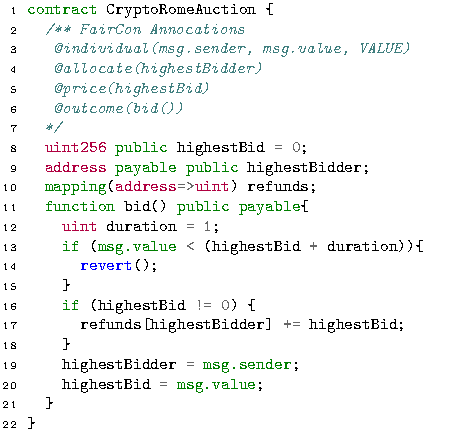
\includegraphics[width=.9\columnwidth]{Figures/Chapter3/auction.pdf}
  \caption{The CryptoRomeAuction Solidity source code.}\label{CryptoRomeAuction}
\end{figure}


%\begin{comment}
%\begin{figure}[t]
%  \small
%  \begin{align*}
%    & \texttt{CryptoRomeAuction} := (msgsender_1, msgvalue_1, \_ ) \\
%    & \quad (msgsender_2, msgvalue_2, \_ ) \\
%    & \quad (msgsender_3, msgvalue_3, \_ ) \\
%    & \quad (msgsender_4, msgvalue_4, \_ ) \\
%    & \quad (msgsender_5, msgvalue_5, \_ ) \\
%    & \quad \texttt{\textbf{assume}}:\; (\mnot (msgvalue_2 < msgvalue_1 + 1)) \mand \\
%    & \quad\quad (\mnot (msgvalue_3 < msgvalue_2 + 1)) \mand \\
%    & \quad\quad (\mnot (msgvalue_4 < msgvalue_3 + 1)) \\
%    & \quad \texttt{\textbf{allocate}}:\; \texttt{\textbf{argmax}}(msgvalue_1,
%    msgvalue_2, msgvalue_3,\\
%    & \quad\quad msgvalue_4,msgvalue_5)\\
%    & \quad \texttt{\textbf{price}}:\; \texttt{\textbf{max}}(msgvalue_1, msgvalue_2,
%    msgvalue_3,\\
%    & \quad\quad msgvalue_4,msgvalue_5)
%\end{align*}%
%  \caption{The mechanism model of CryptoRomeAuction with five bidders.}\label{Crypto_Mechanism}
%\end{figure}
%\end{comment}
\paragraph{Threats to Contract Fairness}
One way that \texttt{CryptoRomeAuction} can become unfair to the participants is through the so
called \emph{shill bidding}~\cite{jenamani2007cheating}---a shill tries to escalate the price
without any intention of buying the item.
This can be induced by either the auctioneer or adversarial participants, and other bidders may
need to pay more as a result.
Occasionally, the shill wins the auction if no other higher bid comes before auction ends.
The item may then be sold again at a later time.

\begin{table}[t]
  \caption{Example instances of CryptoRomeAuction.}\label{tab:example}
  \centering\small
  \begin{tabular}{l|ccc|ccc|ccc}
    \toprule
    & \multicolumn{3}{c|}{Truthful} & \multicolumn{3}{c|}{Untruthful} &
    \multicolumn{3}{c}{Collusion} \\
    \midrule
    Bidder & $p_1$ & $p_2$ & $p_3$ & $p_1$ & $p_2$ & $p_3$ & $p_1$ & $p_2$ & $p_3$ \\
    \midrule
    Valuation  & 3 & 4 & 6 & 3 & 4 & 6 & 3 & 4 & 6\\
    Bid  & 3 & 4 & 6 & 3 & 4 & 5 & 3 & 0 & 4 \\
    Allocation  & \xmark & \xmark & \cmark & \xmark & \xmark & \cmark & \xmark & \xmark & \cmark \\
    Price & 0 & 0 & 6 &  0 & 0 & 5 & 0 & 0 & 4 \\
    Utility  & 0 & 0 & 0 & 0 &  0 & 1 & 0 & 1 & 1 \\
    \bottomrule
  \end{tabular}
\end{table}

Apart from shill bidding, there are a number of other well-studied properties from the game theory
and mechanism design literature, which can be used to evaluate the fairness of an auction.
We use the example instances shown in \cref{tab:example} to demonstrate.
Suppose there are three bidders, $p_1$, $p_2$, and $p_3$, participating in the auction.
Each of them has a valuation of the item, i.e., the item worth three, four, and six units of utility for
$p_1$, $p_2$, and $p_3$, respectively.
The Columns ``Truthful'', ``Untruthful'', and ``Collusion'' in \cref{tab:example} show the
three example scenarios, where the players act truthfully, untruthfully, and collude among
themselves.
The Rows ``Bid'', ``Allocation'', ``Price'', and ``Utility'' show the bids placed, the final
allocation of the item, the clear price, and the utilities obtained by the bidders, respectively.

Same as other first-price auction schemes, \texttt{CryptoRomeAuction} is not \emph{truthful}, i.e.,
bidding truthfully according to one's own valuation of the item is not a dominant strategy.
%Here we show a bidder can cheat in since $CryptoRomeAuction$ cannot have positive incentive to
%drive bidder to truthfully report his bid price.
%Consequently, that cheating bidder could make higher utility while the auction seller suffer the
%loss.
In the ideal truthful scenario, all bidders bid according to their valuations, and $p_3$ wins the
bid with a utility of zero, because the payment equals to his/her valuation of the item.
In another scenario, where $p_3$ bids five (untruthfully), his/her utility would increase by one because
of the lower clear price.
This is called \emph{bid shading}, which only affects the revenue from the auction in this example,
but may affect other participants' utilities in some other cases.
%Further, this cheating benefit may bring negative incentive to other bidders to exercise their
%own truthful bid for this auction as well, which could damage the social welfare realizing in the
%auction.

In the third scenario, $p_2$ and $p_3$ collude in order to gain extra profits.
With full knowledge of each other's valuations, $p_2$ and $p_3$ may decide to form a cartel and
perform bid shading.
One possibility is to have $p_2$ forfeit his/her chance and $p_3$ bids four, and they divide the
profit equally among themselves.
Each of them gains one unit of utility as a result.

%Similar to this example, we also had found cheating problem widely exists in smart contract even
%though there exist many well designed truthful mechanisms available. Unfortunately, many auction
%smart contract try to give a fair illusion to users either via having a promising name or via
%exaggerating its functionality, in order to attract more users involved in the smart contract.
%Meanwhile, the opacity of fairness property of smart contract might make potential users unwilling
%to participate in auction smart contract, thereby decreasing possible social welfare further. Upon
%knowing the fairness properties of auction or other similar type of smart contract,  user may make
%reasonable decision to participate or not in the smart contract.

\paragraph{Checking Fairness Properties}
%\yi{We need to talk about (high-level) how to check fairness properties, such as collusion, on this example automatically.}
Given a mechanism model abstracting the auction settings, the set of fairness properties are
well-defined and can be formally specified based on the model.
The main challenge remains on how to extract the underlying mechanism model from the smart contract
source code.
Now we illustrate how this is done for \texttt{CryptoRomeAuction} in \tool and outline the process
of automated property checking as well as verification.

%An auction smart contract can be seen as one implementation of some mechanism. To evaluate whether
%auction contract enables truthful incentive or not, we should observe the input and outcome of
%auction related mechanism.
Albeit variations in implementations, all auction contracts share some common components, such as
the bidders' identifiers, their bids, and the allocation as well as clear price rules.
We rely on users to provide annotations for these components directly on the source code, which are
demonstrated on Lines 2--7 in \cref{CryptoRomeAuction}.
Specifically, the annotations specify the bidders' information as a tuple,
``\texttt{@individual(msg.sender,msg.value)}'', indicating the variables used to store the
identifier and the bid value, respectively.
Similarly, ``\texttt{@allocation(highestBidder)}'' and ``\texttt{@price(highestBid)}'' indicate
that the allocation result and the clear price are stored in \texttt{highestBidder} and
\texttt{highestBid}, respectively.
Finally, ``\texttt{@outcome}'' is used to label the function defining the auction allocation logic.

\begin{figure}[t]
  \small
  \begin{align*}
  & \texttt{CryptoRomeAuction} := (msgsender_1, msgvalue_1, \_ ) \\
  & \qquad (msgsender_2, msgvalue_2, \_ ) \\
  & \qquad (msgsender_3, msgvalue_3, \_ ) \\
  & \qquad \texttt{\textbf{assume}}:\; (\mnot (msgvalue_2 < msgvalue_1 + 1)) \mand \\
  & \qquad\qquad (\mnot (msgvalue_3 < msgvalue_2 + 1)) \\
  & \qquad \texttt{\textbf{allocate}}:\; \texttt{\textbf{argmax}}(msgvalue_1,
  msgvalue_2, msgvalue_3)\\
  & \qquad \texttt{\textbf{price}}:\; \texttt{\textbf{max}}(msgvalue_1, msgvalue_2,
  msgvalue_3)
  \end{align*}%
  \caption{The mechanism model of CryptoRomeAuction with three bidders.}\label{Crypto_Mechanism}
\end{figure}

With these labels, we perform symbolic execution~\cite{king1976symbolic} on the \texttt{bid()}
function treating the participants' inputs---\texttt{msg.value}---as \emph{symbolic variables}.
The result of this would be two symbolic expressions for both \texttt{highestBidder} and
\texttt{highestBid}, which symbolically represent the allocation and clear price functions,
respectively.
We can then use these information to synthesize an intermediate mechanism model, shown in
\cref{Crypto_Mechanism}.
The model is specified in a customized language designed for auction and voting contracts.
Details of the language syntax and semantics can be found in \cref{section:mechanism_property}.
At the high level, the model specifies information of the participating individuals and the auction
rules: we consider a bounded model with only three bidders (i.e., $msgsender_1$, $msgsender_2$, and
$msgsender_3$), their bids have to satisfy the constraint specified in the \texttt{assume} clause,
the allocation function is given as ``$\argmax(msgvalue_1,\allowbreak msgvalue_2,\allowbreak
msgvalue_3)$'', and the clear price function is given as ``$\max(msgvalue_1,\allowbreak
msgvalue_2,\allowbreak msgvalue_3)$''.


%In our example as shows in Table \ref{tab:example}, the bid price is the
%input while allocation and payment are parts of the outcome. However, we cannot rely on observing
%the simple input and outcome to reason the fairness property because the valuation of bidder is
%ignored when generating the outcome but useful when analyzing the outcome.
The intermediate mechanism model in \cref{Crypto_Mechanism} has well-defined mathematical
semantics, which can be used to check the desired fairness properties.
We encode both the model and the property with an SMT formula such that a counterexample exists if
and only if the formula is satisfiable.
More details on the encoding can be found in \cref{subsection:property_checking}.
If the formula is unsatisfiable, we are confident that the property holds for the bounded case with
three bidders.
We then attempt to prove the property by instrumenting the contract program with \emph{program
invariants} encoding the allocation and clear price clauses synthesized previously, but
parameterized by an unbounded number of bidders.
The instrumented program and the property are then passed to a program verification tool, such as
Dafny~\cite{dafny}, to perform the automated verification.

%Having the valuation in
%analyzing process, taking $CryptoRomeAuction$ as example, firstly we assume there are some players
%that successively update the current highest bidder, then next comes two situation: $M$ $M'$. M is
%ideally truthful for every bidder and we get the utility $u$ of last bidder, the winner in this
%scenario, $M'$ is truthful for every bidder but the last bidder,and we get the utility $u'$ of last
%bidder, also the winner in this scenario, Next comes the comparison between $u$ and $u'$. If $u'$
%is larger than $u$, we can conclude that the contract fails the truthfulness property.  Otherwise,
%we may have some confidence of the truthfulness property of the contract and need to verify it
%using invariant reduction that will discussed in Section \ref{Sec_Method}.











\section{The Analysis Framework for Smart Contract Fairness}
\label{section:mechanism_property}

\textcolor{red}{Provide a general introduction and overview of the materials/methods and supply essential background information}

In this section, we first provide necessary background and definitions on mechanism models and
fairness properties well studied in the mechanism design
literature~\cite{jackson2014mechanism,nisan2001algorithmic}.
Then we give the abstract syntax and semantics of our mechanism modeling language to support
automated model construction and property checking.

\subsection{Smart Contracts as Mechanism Models}\label{sec:mechanism-model}
Mechanism design is used to design economic mechanisms or incentives to help attain the goals of
different stakeholders who participate in the designated activity.
The goals are mainly related to the outcome that could be described by participants' payoff and
their return in the activity.
We model the logic behind smart contracts with a mathematical object known as the mechanism.
%Largely because of many existing diverse definitions, here we formally describe the mechanism model
%for later understanding fairness property, without the loss of generality.

In a \emph{mechanism model}, we have a finite number of individuals, denoted by $N = \{1, 2, \ldots,
n\}$.
Each individual $i$ holds a piece of private information represented by a \emph{type}, denoted
$\theta_{i} \in \Theta_i$.
Let the types of all individuals be $\theta = (\theta_1, \ldots, \theta_n)$, and the space be
$\Theta = \times_i \Theta_i$.
The individuals report, possibly dishonestly, a \emph{type (strategy) profile} $\report \in \Theta$.
Based on everyone's report, the mechanism model decides an outcome which is specified by an
\emph{allocation function} $d: \Theta \mapsto O$, and a \emph{transfer function} $t: \Theta \mapsto
\mathbb{R}^n$, where $O = \{o_i \in \{0,1\}^n \mid \Sigma_i o_i = 1\}$ is the set of possible
outcomes.

The preferences of an individual over the outcomes are represented using a \emph{valuation function}
$v_i: O \times \Theta_i \mapsto \mathbb{R}$.
Thus, $v_i(o, \theta_i)$ denotes the benefit that individual $i$ of type $\theta_i$ receives from an
outcome $o \in O$, and $v_i(o,\theta_i) > v_i(o',\theta_i)$ indicates that individual $i$ prefers
$o$ to $o'$.
%Individuals may also need to make or receive payment, which is defined by a \emph{transfer
%function}
%$t_i: \Theta \mapsto \mathbb{R}$.
%\yi{TODO: some notations need to be fixed.}
%Having the benefit function $v$ over decisions and transfer
%function $t$, we can easily get the utility $u_i$ of the individual $i$: $ u_i(\theta) =
%v_i(d(\theta), \theta_i) - t_i(d(\theta), \theta_i^s)$. and the social welfare $W$ is sum of all
%individuals' utilities: $ W = \sum_{i=1}^n u_i(\theta)$.
The individual $i$'s utility under strategy profile \report is calculated by subtracting the
payment to be made from the valuation of a certain outcome: $u_i(\report) = v_i(\report,
\theta_i) - t_i(\report)$.

%A \emph{strategy} is a mapping from types to
%For simplicity, we also directly use $\theta_i^s$ to refer to individual's strategy to report his
%type.
%Generally, every individual has his own private information type independent of each other;
%We would use pair ($\theta_i$, $\hat{\theta_i}$) to represent the strategy to truthfully report
%individual's type and the strategy to untruthfully report individual's truthful type respectively,
%where $\theta_i \in \Theta_i$ and $\hat{\theta_i} \in \Theta_i$, $\Theta_i$ are the set of all
%strategies for individual $i$;

%Let $\theta = (\theta_1^s,\theta_2^s,\dots,\theta_n^s)$ be all individual's strategies, $\theta
%\in \Theta$ and
%$\theta_i^s \in \Theta_i$. Mechanism model takes as input individuals' strategies $\theta$ and as
%output an outcome $\Octon$ generated by a common social decision function $d(\theta)$ across
%individuals and a set of transfer function $t(d(\theta),\theta_i^s)$ for individual $i$. For
%social
%decision function $d(\theta) \in D$, where $D$ is the set of all possible social decisions made
%among the individuals. The transfer function $t(d(\theta),\theta_i)$ is to calculate, based on the
%decision $d(\theta)$ and $\theta_i$, the strategy of individual $i$, how much individual $i$
%should
%pay.

%\begin{definition}[Mechanism Model]
%A mechanism model $(N, \report, O)$ is described by a set of individuals $N$ and their input
%strategies $\theta$ and an outcome $\Octon$ subjects to a social decision function
%$d(\theta)$:$\Theta \rightarrow \N $ and a transfer function $t(d(\theta))$:$\Theta \rightarrow
%\R^n$. We denote as $t_i(d(\theta),\theta_i^s)$ the transfer for individual $i$.
%\end{definition}

%Furthermore, for any individual, which his strategy is would affect the decision afterwards and how
%much he should pay on that decision.
%So basically each individual has its preference over different social decisions.
%We use the benefit function $v_i(d(\theta), \theta_i)$ to denote the benefit value for the
%individual $i$ from the decision generated by $d(\theta)$.

\subsection{Fairness Properties}\label{subsec:FairnessProperty}
%\yi{Need to talk about why these properties.}
%\liu{ Fairness is a meaningful but broad problem of software development. Fairness itself seems to
%be generally subjected to different domains knowledge.}
%\liu{For most of the mechanism design practice, the need of a truthful-incentive mechanism ranks
%at the top,
%meanwhile keeping the mechanism efficient for user to participate and optimal for the mechanism
%stakeholders to benefit, the so-called maximizing the social welfare, also
%matter~\cite{jackson2014mechanism}.
%Moreover, a good mechanism design should resist against users' collusion~\cite{wu2018cream}.
%These needs or features construct mechanism fairness to some extent.
%}
The fairness of smart contracts is usually subject to the understandings and preferences of the
participating parties---a contract fair to someone may be unfair to the others.
In particular, fairness can be considered from both the participants' and the contract creators'
points of view.
To capture such nuances, individual parties have to be modeled separately before such subjective
fairness properties can be specified against the model.

Generally speaking, all properties which can be expressed in terms of the mechanism model defined
in \cref{sec:mechanism-model} are supported by our reasoning framework.
To keep the presentation simple, in this paper, we focus on analyzing a set of generic fairness
properties based on the mechanism models.
%\liu{The mechanism model itself can be used to model and verify fairness of any	game-like smart
%contract involving multiple participants.}
We restrict the discussion to four types of well-studied properties in the literature, namely,
truthfulness, optimality, efficiency, and collusion-freeness.

%\liu{These fairness properties matter a lot to smart contract. }
%\begin{comment}
%from 2-collusion mechanism to collusion-freeness fairness property, we may need a discussion to
%explain the gap. Because the gap acutally exists and matters.
%\end{comment}

To formally define the properties, we first introduce an important concept---\emph{dominant
strategy}.
We use $\report_{-i}$ to denote the strategy profile of the individuals other than $i$, i.e.,
$(\report_1, \ldots, \report_{i-1},\allowbreak \report_{i+1},\allowbreak \ldots,\allowbreak
\report_n)$.
Therefore, $(\report_i', \report_{-i})$ is used to denote the strategy profile which differs from
\report only on $\report_i$.

\begin{definition}[Dominant Strategy]
  A strategy $\report_i \in \Theta_i$ is a dominant strategy for $i$, if $\forall
  \report_{-i} \forall \report_i' \in \Theta_i \cdot u_i(\report_i, \report_{-i}) \geq
  u_i(\report_i', \report_{-i})$.
  When equality holds, the strategy is a weak dominant strategy.
\end{definition}

We say that a mechanism model is truthful if and only if for any individual and strategy profile,
reporting one's real type (truth-telling, i.e., $\forall i \in N \cdot \report_i = \theta_i$) is a
dominant strategy.

\begin{definition}[Truthfulness]\label{def:truthful}
  Formally, a mechanism is truthful if and only if,  $\forall \theta_{-i} \forall \report_i \in
  \Theta_i \cdot u_i(\theta_{i}, \theta_{-i}) \geq u_i(\report_i, \theta_{-i})$.
\end{definition}
%<<<<<<< HEAD
%
%In an auction contract, the account which creates the auction is the \yi{beneficiary?} and the
%accounts which join the auction are the bidders.
%\yi{If the auction prevents bidders from gaining more by bidding less, it is said to be truthful.}
%Since bidding untruthfully is not a good strategy, truthful auctions can generally attract more
%honest participants so that the \yi{beneficiary?} can get much higher revenue for the item sold.
%=======
Given an auction smart contract with many bidders competing for a single indivisible good, the
account which creates the contract is the \emph{auctioneer} and the accounts which join the auction
are the \emph{bidders}.
If the auction prevents bidders from benefiting more by bidding less, it is truthful.
When bidding untruthfully is not a good strategy, the auction can generally attract more honest
bidders and the auctioneer can get higher revenue for the good on sale.


\begin{definition}[Efficiency]
  We say a mechanism is efficient if and only if its allocation function achieves maximum total
  value, i.e., $\forall \report \in \Theta \forall d' \cdot \sum_{i} v_{i}(d(\report), \theta_{i})
  \geq \sum_{i} v_{i}(d'(\report)$, $\theta_{i})$.
\end{definition}

Suppose no bidder can affect any other bidder's valuation.
If the only winner is the bidder who values the good the most, the auction is efficient.

\begin{definition}[Optimality]
  We say a mechanism is optimal if and only if its transfer function achieves maximum total net
  profit, i.e., $\forall \report \in \Theta \forall t' \cdot \sum_i t_i(\report) \geq
  \sum_i t_i'(\report)$.
\end{definition}

Similarly, if the winner is the one who bids the highest, the auction is optimal.
In this case, the auctioneer receives the highest revenue.

We use $\report_{-ij}$ to denote the strategy profile of individuals other than $i$ and $j$, i.e.,
$\{\report_1, \allowbreak \ldots, \allowbreak \report_{i-1}, \allowbreak \report_{i+1}, \ldots,
\report_{j-1}, \report_{j+1}, \allowbreak \dots, \report_n\}$.

\begin{definition}[2-Collusion Free]
  We say a mechanism is 2-collusion free if there does not exist a cartel of individuals $i$ and
  $j$, whose untruthful strategies increase the group utility, formally,
  $u_i(\hat{\theta_i}, \allowbreak \hat{\theta_j}, \allowbreak \theta_{-ij}) + u_j(\hat{\theta_i},
  \hat{\theta_j},\theta_{-ij}) \geq u_i(\theta_i, \allowbreak \theta_j, \allowbreak \theta_{-ij}) +
  u_j(\theta_i, \theta_j, \theta_{-ij})$.
\end{definition}
%<<<<<<< HEAD
%\liu{Above we present 2-Collusion free property.
%Briefly, if \texttt{Auction} can prevent any two bidders collusion by making their collusion gains
%not greater than their non-collusion gains, we say \texttt{Auction} is 2-collusion free, which
%could prevent bid price manipulation to some extent so as to realize higher revenue for its
%beneficer.}
%\yi{How about n-collusion free?}
%=======
Collusion is a big concern in auction and other multi-player games.
The basic 2-collusion freeness property in an auction means that any two bidders' collusion cannot
help them achieve higher gain.
This prevents bid price manipulation to a certain extent, which helps guarantee fair chance for all
bidders and maintain good revenue for the auctioneer.
A more general version, i.e., $n$-collusion freeness, can be defined in a similar way.
%>>>>>>> save fixes
%\lstset{numbers=none}
%Based on syntax given in Sect.~\ref{subsection:syntax}, we make some extension to the syntax and
%Fig.~\ref{syntax} draws the description language for the four fairness properties.

%\yi{Give intuitions about these definitions.}


\subsection{Mechanism Modeling Language}\label{subsection:syntax}

We now propose a domain-specific language to facilitate the automated translation from smart
contracts to mechanism models.


\begin{figure}[t]
\small
\begin{align*}
  \texttt{<individual>}  &:= (id: \mathbb{S}, bid: \N, val: \N ) \\
  \texttt{<func>}        &:= \texttt{\textbf{max}} \;|\; \texttt{\textbf{argmax}} \\
  \texttt{<exp>}         &:= \texttt{<individual>}.id \;\;|\;\; \texttt{<individual>}.bid \\
                         &\;\;|\;\; \N \;\;|\;\; \texttt{<exp> \texttt{[+-]} <exp>}
                          \;\;|\;\; \texttt{<func>(<exp>*)} \\
  \texttt{<bool>}        &:= \texttt{<exp> == <exp>} \;\;|\;\; \texttt{<exp> < <exp>} \\
                         &\;\;|\;\; \mnot \texttt{<bool>} \;\;|\;\; \texttt{<bool>}
                          \mand \texttt{<bool>} \\
  \texttt{<assumption>}  &:= \texttt{\textbf{assume}} : \texttt{<bool>} \\
  \texttt{<outcome>}     &:= \texttt{\textbf{allocate}} : \texttt{<exp>} \\
                         &\;\;|\;\; \texttt{\textbf{price}} : \texttt{<exp>}; \;
                          \texttt{\textbf{allocate}} : \texttt{<exp>} \\
  \texttt{<property>}    &:= \texttt{<bool>} \;\;|\;\; \texttt{\textbf{forall}} : \texttt{<bool>} \\
  \texttt{<mechanism>}   &:= \texttt{<individual>*}; \; \texttt{<assumption>}; \;
                          \texttt{<outcome>}; \\
                         &\quad\;\; \texttt{<property>}
\end{align*}%
\caption{Syntax of the auction/voting mechanism model.}\label{syntax}
\end{figure}

We define an abstract syntax of the mechanism modeling language, which is applicable to both auction
and voting.
\Cref{syntax} shows the context-free grammar of the language.
A mechanism model comprises one or more \emph{individuals}, an \emph{assumption}, an
\emph{outcome}, and a \emph{property} to be verified.
An individual is defined as a triple containing the identifier ``$id$'', bid amount ``$bid$'', and
valuation ``$val$''.
An assumption is a Boolean constraint which should be satisfied upon the entry of the contract.
The outcome of the contract is specified by the allocation and the clear price functions, which are
expressions over $id$ and $bid$.
Voting contract typically does not have a clear price function.
We allow properties to be specified using a Boolean expression optionally preceded by a ``forall''
quantifier.

\begin{figure}[t]
  \AxiomC{$(id_1,bid_1,val_1), \ldots, (id_n,bid_n,val_n)$}
  \RightLabel{[Indiv]}
  \UnaryInfC{\stackanchor{$N \leftarrow \{1, \ldots ,n\}$ \quad $\report \leftarrow%
      \{bid_1,\ldots,bid_n\}$}%
    {$\{v_i(o_i, \theta_i)\} \leftarrow \{val_i\}$}}
 
  \DisplayProof \vskip .1in
  \AxiomC{$\texttt{\textbf{assume}}:assumption$}
  \AxiomC{$\texttt{\textbf{allocate}}:allocation$}
  \RightLabel{[Alloc]}
  \BinaryInfC{$d(\report) \leftarrow \textbf{eval}(assumption \wedge allocation)$}
  \DisplayProof \vskip .1in
  \AxiomC{$\texttt{\textbf{assume}}:assumption$}
  \AxiomC{$\texttt{\textbf{price}}:clearprice$ }
  \RightLabel{[Price]}
  \BinaryInfC{$t(\report) \leftarrow \textbf{eval}(assumption \wedge clearprice)$}
  \DisplayProof
  \caption{Semantic rules of the auction/voting model.}\label{semantics}
\end{figure}

\begin{figure*}[!t]
  \centering
  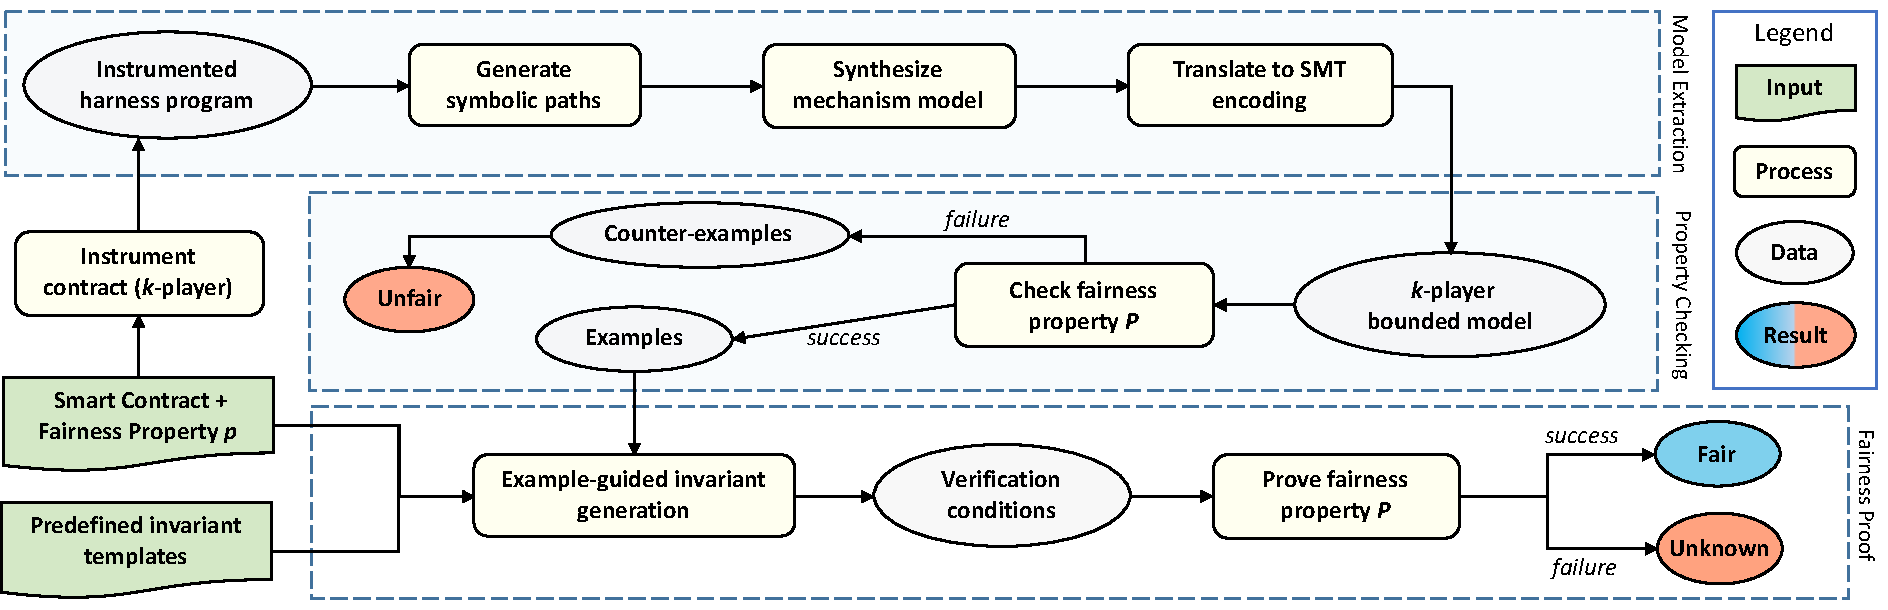
\includegraphics[width=\textwidth]{Figures/Chapter3/framework.pdf}
  \caption{Workflow of the \tool framework.}\label{fig:framework}
\end{figure*}

\paragraph{Language Semantics}
The semantic mapping from the modeling language to the underlying mechanism model is summarized in
\cref{semantics}.
The ``Indiv'' rule maps the individuals and their reported types as well as valuations.
More specifically, the individuals' bids are mapped to their reported types \report, and an
individual of type $\theta_i$'s valuation of the item $v_i(o_i, \theta_i)$ is $val_i$, where $o_i$
denoted the outcome where the item is allocated to $i$.
The ``Alloc'' rule conjuncts the Boolean expression $assumption$ from the ``assume'' clause and the
symbolic expression $allocation$ in terms of individuals' strategies from the ``allocate'' clause,
which is evaluated as the allocation function.
Similarly, the transfer function is the conjunction of the $assumption$ and the $clearprice$
expressions.

There are some differences between auction and voting:
clear price is absent from voting, where allocation is done by comparing the number of ballots
(bids) by the participating individuals;
%Above we only present the outcome semantic rule for the auction.
whereas in auction, the individuals who bid no less than the clear price can be allocated the item.

This language works for the most commonly seen auction and voting contracts with fairness concerns.
For example, Ethereum smart contracts meeting the ERC-1202 (voting)~\cite{erc-1202} and ERC-1815
(blind auctions, under review)~\cite{erc-1815} standards all follow the same interface and
structure, therefore can be automatically translated into our modeling language.
Similar languages can also be designed for other types of contracts (e.g., social games).
The proposed modeling language can be modified and extended to establish suitable mappings from new contract types to the classic mechanism model.
With the new modeling language, the model extraction and property checking algorithms can be
directly reused.


\section{The \tool Framework}\label{Sec_Method}
\textcolor{red}{Restate the purpose of the work and provide specific and precise details about source of materials and methods}
%In the section 3, we have illustrated the mechanism model and also specified the
%four important fairness properties.

In this section, we present the \tool verification framework for smart contract fairness.
\Cref{fig:framework} shows the overall workflow of \tool.
The framework consists of three modules, namely, \emph{model extraction}, \emph{property checking},
and \emph{fairness verification}.

The smart contract source code is first automatically instrumented according to user-provided
annotations.
At this stage, we consider a $k$-player bounded model, and the instrumented contract code contains
a harness which orchestrates the interactions between the players and the target contract.
The extraction of the mechanism model is powered by symbolic execution of the harness program, and
an intermediate mechanism model is synthesized as a result.
%First one is symbolic execution of smart contract at source-code level, which is supported by the
%custom symbolic engine.

In order to perform property checking, the intermediate mechanism model, along with the desired
property, are encoded as an SMT formula, such that the formula is unsatisfiable if and only if the
property holds with respect to the model.
We use an SMT solver to check and may declare the property holds when the number of participants
are bounded by $k$; otherwise, a counterexample is generated which disputes the property.
%Next comes the property checking part, where our goal is to reveal some unfair
%smart contract by observing counterexample generated, which violates the fairness property.
%If the symbolic execution cannot generate counterexample, we manually use invariant-like technique
%to explore function scheme or say phase scheme related to mechanism design, to abstract smart
%contract, and then based on these abstract schemes, verify whether fair property holds or not
%without any misleading results.

If we fail to find a counterexample in the bounded case, we may proceed to the fairness
verification of the properties for unbounded number of participants.
To do that, we modify the harness to account for an unlimited number of players, instrument it with
program invariant as well as the desired properties as post-conditions, and rely on program
verification tools to discharge the proof obligations.
This either tells us that the property is successfully proved, or the validity of the property is
still unknown, in which case we are only confident about the fairness for the bounded case.


\subsection{Mechanism Model Extraction} \label{subsec:ModelExtraction}

\begin{figure}[t]
\centering
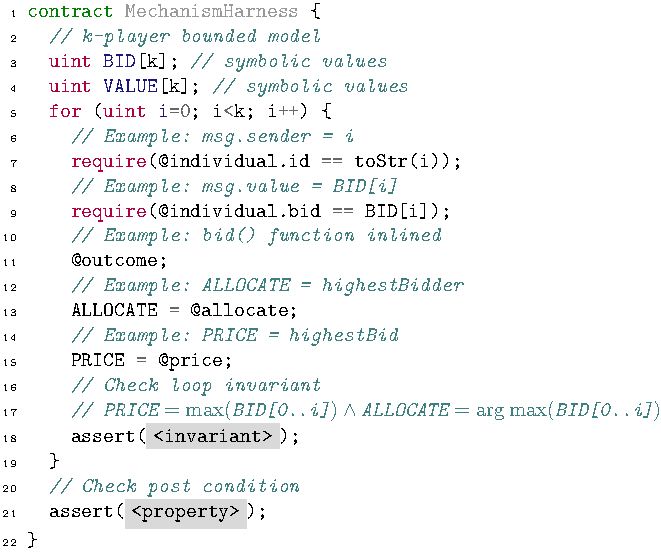
\includegraphics[width=\columnwidth]{Figures/Chapter3/harness.pdf}
\caption{The harness program for mechanism model orchestration.}\label{fig:harness}
\end{figure}

%For smart contract, it has no limitation to the number of participants, since
%the smart contract has a dynamic mechanism model that could involve a lot of
%participants, which is difficult to manually analyze fairness properties on the
%smart contract. In most times, It is also difficult to analyze fairness property
%of complicated smart contract with even a small number of participants. So we
%propose a prototype tool Solse+ to automatically check fairness properties on the
%smart contract. Our tool can help: (1) developers to have an idea of fairness about
%their smart contracts from the perspective of the mechanism. (2) participants to
%be cautious to attend unfair smart contracts.

To extract a mechanism model out of the smart contract source code, we first instrument the
contract code with a harness program \texttt{MechanismHarness} shown in \cref{fig:harness}.
The harness program orchestrates the interactions of $k$ players with the target contract.
This is achieved by declaring symbolic variables to represent the possible bid and valuation of
each player, stored in the arrays ``\texttt{BID}'' (Line 3) and ``\texttt{VALUE}'' (Line 4),
respectively.
Then a for-loop (Lines 5--19) is used to simulate the actions performed by the $k$ players.
In smart contract, all players have to move sequentially since parallelization is not allowed.
The ordering is not important, because the players are symmetric.

We rely on the annotations provided by users (e.g., \cref{CryptoRomeAuction}) to construct the
loop body, which triggers a move from one particular player.
The variables controlling the player's identifier and bid value are assigned the corresponding
symbolic values (Lines 7 and 9).
In the case of \cref{exp:cryptorome}, these variables are \texttt{msg.sender} and
\texttt{msg.value}, respectively.
Then the allocation function (e.g., \texttt{bid()} in \cref{exp:cryptorome}) is inlined, and
the resulting variables annotated by \texttt{@allocate} and \texttt{@price} are stored as symbolic
expressions (Lines 13 and 15).
There are also two placeholders at Lines 18 and 21, for assertions of loop invariant and post
conditions, which will be described in \cref{subsection:formal_proof}.

We then run symbolic execution on the harness program to collect a set of feasible symbolic paths.
Each symbolic path is represented in the form of ``$\mathit{Condition} \wedge \mathit{Effect}$'',
where ``$\mathit{Condition}$'' and ``$\mathit{Effect}$'' are Boolean expressions in terms of the
symbolic variables defined earlier (e.g., \texttt{BID[i]} and \texttt{VALUE[i]} in
\cref{fig:harness}).
Here, ``$\mathit{Condition}$'' represents the \emph{path condition} which enables the execution of a
particular program path; ``$\mathit{Effect}$'' represents the values of the resulting variables
(e.g., \texttt{ALLOCATE} and \texttt{PRICE} in \cref{fig:harness}).
We take all path conditions $\mathit{Condition}_j$, where the effect is successfully computed
(i.e., not running into errors or reverts), and use the disjunction of them as the
$\mathit{assumption}$ of the model (i.e., ``\texttt{assume} $\bigvee_j \mathit{Condition}_j$'').
Similarly, we use the effects as the corresponding allocation and clear price functions.
For example, in the mechanism model, we have ``\texttt{allocate} $\bigvee_j (Condition_j \wedge
\mathit{Effect}_j[ALLOCATE])$'' and ``\texttt{price} $\bigvee_j (\mathit{Condition}_j \wedge
\mathit{Effect}_j[PRICE])$''.

%Our tool Solse+ can check all possible collected symbolic paths.
%If there is checking failure on one path, the Solse+ will generate relevant counterexample for this
%path.
%The counterexample could also be deemed as an instance of the mechanism model of the smart contract
%in our context.
%
%We also have an extension integrated with our tool to support the analysis of the mechanism model.
%This extension covers the variable notation function of the participants or so-called individuals.
%So Solse+ not only collects a symbolic path of smart contract but also collected the mechanism
%components and related fairness property expression.
%For simplicity, Solse+ first removes the unreachable paths


\subsection{Bounded Property Checking}\label{subsection:property_checking}
%\begin{comment}
%\textcolor{red}{Formal representation to fairness property checking problem}
%\begin{itemize}
%    \item  model formalization using formal notation
%    \item  different validity of property on mechanism model
%    \item  technical challenge
%    \item  taking mentioned example to illustrate how to check
%\end{itemize}
%\textcolor{red}{Fairness property analysis}
%\begin{itemize}
%    \item  present simple ground truth where mechanism is untruthful
%    \item  present simple ground truth where mechanism is truthful
%\end{itemize}
%\end{comment}
%Once our tool recovers the mechanism model out of the smart contract, we can get the boolean
%expression of fairness properties and then check whether this expression can attain true value.
%Here we simply formalize the checking process for our fairness properties.

For property checking, given a mechanism model $M$ and a property $p$, our goal is to construct a
formula $\phi$ such that $\phi$ is unsatisfiable if and only if $M \models p$.
With the semantic rules defined in \cref{subsection:syntax}, it is straightforward to obtain a
formula encoding the allocation and clear price functions, i.e., $\varphi_M = d(\theta) \wedge
t(\theta)$.

We illustrate the encoding of properties using the truthfulness as an example.
\Cref{def:truthful} states that a model $M$ is truthful if and only if the truth-telling
strategy performs no worse than any other strategies.
Therefore, the high-level idea is to first encode the truthful and untruthful strategies separately
for an arbitrary player, and then asserting that the utility of the player is higher when he/she
acts untruthfully.
The encoding of the truthfulness property $p$ is shown as follows,%
\begin{align*}
\exists i \cdot & \forall j \cdot (i \neq j) \implies \\
& (\varphi_M \land (bid_i = val_i) \land (bid_j = val_j)) \tag{Truthful} \\
\land\; & (\varphi_M[bid_i/bid_i', u_i/u_i'] \land (bid_i' \neq val_i)) \tag{Untruthful} \\
\land\; & (u_i < u_i'), \tag{Utility}
\end{align*}%
where $i$ is a generic player with utility $u_i$.
The truthful scenario is when all players (including $i$) bid the same amount as their valuations,
i.e., $bid_i = val_i$ and $bid_j = val_j$.
The untruthful model is constructed by substituting the bid and utility variables of $i$ with new
copies $bid_i'$ and $u_i'$, and asserting $bid_i' \neq val_i$.
Finally, we assert that $u_i < u_i'$.
If $p$ is satisfiable, we find a counterexample where an untruthful strategy performs better than
the truthful strategy.
Otherwise, the truthful strategy is a dominant strategy for $i$.
The encodings of other properties are similar.
%Using the abstract syntax of a mechanism model, we could can denote a mechanism model using the
%notation $\phi: \{I, O\}$,
%where $I(x)$ refers to the individuals related information of a mechanism model,
%and $O(I(x))$ refers to the outcome of the mechanism given $I(x)$. Let  $\varphi$ be the fairness
%property, we can describe a particular property $\varphi$ of a given mechanism model $\phi$.
%$\phi$ could be simplified as $ \phi = O(\forall x I(x))$.

%We say a property $\varphi$ holds for a given mechanism model $\phi$ iff $ \varphi(\phi)
%\rightarrow \nexists O'\forall x \varphi(O'(I(x)))$ or $ \varphi(\phi) \rightarrow \forall x
%\varphi(O(I(x)))
%$. This means a property holds for a given model no matter what the participants are or its
%outcome function could be improved.

%In the paper, we explore whether the fairness property holds for mechanism model. Due to the
%difficulty of directly checking fairness property
%using symbolic execution on infinite formula, we compromised and checked whether a fairness
%property $\varphi$ holds for a given mechanism model
%under the setting of fixed number of participants.  We say a property $\varphi$ holds for a given
%mechanism model $\phi$ and $k$, the number of $I$ as $\varphi(\phi[\|I\|=k])$. And $
%\varphi(\phi[\|I\|=k])  \Leftrightarrow \nexists O' \forall x \varphi(O(I(x))) \lor \forall x
%\varphi(O(I(x)))$.Obviously, if we found $k$ that make
%property checking fail, we say the mechanism model is not fair w.r.t $\varphi$. On the contrary, we
%say the mechanism model is fair w.r.t $\varphi$ and $k$.
%Subsection \ref{subsection:formal_proof} will illustrate how to prove whether the k-fair mechanism
%model remain fair independent of $k$.
% \begin{figure}[!h]
%   \includegraphics[width=0.45\textwidth]{./figures/MethodTruthfulCheck}
%   \caption{The overview of fairness Property Checking}
%  \end{figure}

%We take truthful property as an example to illustrate our work.
%Assuming a bidder intends to make more profit by cheating on his bid value. This means his actual
%bid value $\hat{\theta}$ will be different from his truthful bid value $\theta$.
%We denote his utility as $u$ and have the following formulas. $ \textMu (\theta) \reduce u_0 $,
%$\textMu (\hat{\theta}) \reduce u_1 $. Truthful property could be expressed as below.
%\[
%    truthful = \begin{cases}
%         False,   & \text{if } u_1 > u_0\\
%         True,     & \text{otherwise}
%    \end{cases}
%\]
%And recall the example $CryptoRomeAuction$ mentioned in Section \ref{section:example}. There are 5
%bidders in the example. Assuming all $5$ bidders'
%value are $\theta_1$, $\theta_2$, $\theta_3$, $\theta_4$, $\theta_5$, only the first bidder intends
%to
%make more profit, so the first bidder would choose the untruthful value $\hat{\theta_1}$. So for
%the first bidder, his utility $u_1$ is as
%\[
%    u_1 = \begin{cases}
%        \theta_1 - \hat{\theta_1},   & \text{if }
%\hat{\theta_1}>max(\theta_2,\theta_3,\theta_4,\theta_5)+duration \\
%         0,     & \text{otherwise}
%    \end{cases}
%\]
%Similarly, if he choose to be truthful, his benefit $u_0$ could be as
%\[ u_0 = \begin{cases}
%       \theta_1 - \theta_1,   & \text{if }
%\theta_1>max(\theta_2,\theta_3,\theta_4,\theta_5)+duration \\
%         0,     & \text{otherwise}
%    \end{cases}
%\]
%Obviously, so long as $\hat{\theta_1}>max(\theta_2,\theta_3,\theta_4,\theta_5)+duration$ and
%$\theta_1 > \hat{\theta_1}$, we can get $u_1 > u_0$, so this smart contract is not truthful.



%Assuming that there is a certain number of bidders participating in an auction, we use our tool to give them different bids repeatedly to check whether they can improve their utility by collusion. Similarly, we also check the \textit{efficiency} property by checking whether the mechanism model can perform the social welfare (the sum of all users’ utilities) maximization.

\subsection{Formal Proof for Unbounded Model}\label{subsection:formal_proof}

%Usually a mechanism model could be logically complicated enough to involve from tens to thousands of participants. To prove fairness property of mechanism model, in case where the participants involved is limited, symbolic execution technique would help checking the property holds or not. However, if the mechanism model allows for significantly large or unlimited participants, the formula generated by the given model instance would be too large to check using symbolic execution. In this case, symbolic execution technique seems not an efficient approach to check the fairness property. Owing to the difficulty to prove whether the fairness property holds for mechanism-enabled smart contract directly using symbolic execution, we resorts to abstract refinement to simplify the mechanism model inside smart contract. And then verify whether fairness property holds for these reduced abstract refinements.


%Generally, allocation and transfer function are essential parts of mechanism model. In nature, allocation function refers to who will win the bid or get the allocated resource, and transfer function refers to how much should be paid for the allocated resource by the winner. We abstract allocation and transfer function respectively from smart contract. Specifically, we find the allocation invariants and transfer invariants separately. Based on the two invariants, we could formally verify those fairness property.

%When we think about social decision function as mentioned in Section \ref{section:mechanism_property}, actually we will care about how the target(s) are allocated. Typically, there are two type of resource for allocation. One is single type of resource allocation such as spectrum allocation, and another one is mixed types of resource allocation such as combinatorial auction. In combinatorial auction, usually multiple types of resources are available for the allocation and targets could be allocated to more than one participants. For simplifying the mechanism analysis for \tool. We limit our focus on single type of resource location without loss of generality of fairness property. Taking into the consideration such diverse scenarios for single type of resource allocation, we attempt to minimize the scenario difference. For instance, First price auction and second price auction are two well-known widely used auction schemes in real world. We can easily make use of their allocation and price forms as the invariants to facilitate verifying fairness property for considerable number of smart contracts that declare to be the type of first price or second price auction.

Consider the harness program in \cref{fig:harness}.
The loop iterates $k$ times to model $k$ players joining in each iteration.
We use induction to prove that the smart contract satisfies the fairness property for arbitrary
number of players.
Following the standard approach to proving program correctness, an invariant for the for-loop is
required, i.e., \texttt{<invariant>} in \cref{fig:harness}.
Normally, the loop invariant has to be derived manually.
Fortunately, smart contracts are usually written in a more standard way than arbitrary programs,
which makes it easier to generalize invariants for the same type of smart contracts, e.g., auctions
considered in this work.
A set of predefined invariant templates (according to specific types of contracts) have to be
provided to the framework as inputs (\cref{fig:framework}).
The followings are three common types of invariants required for auctions.
%We now informally present allocation invariant to facilitate abstracting the essence the
%allocation function hidden in smart contract's mechanism design as well as the price invariants
%for
%the transfer function.
% \begin{figure}[!h]
%   \small
%
%     \textbf{allocation invariants}:
%\vspace{-.4cm}
\begin{flalign}
  \texttt{ALLOCATE}   =& \argmax(\texttt{BID}) \tag{TopBidder} \label{eq:alloc-invariants} \\
  \texttt{PRICE} =& \max(\texttt{BID}) \tag{$1$st-Price} \label{eq:price-invariant1} \\
  \texttt{PRICE} =& \max(\texttt{BID} \setminus \{\texttt{BID}[\argmax(\texttt{BID})]\})
  \tag{$2$nd-Price} \label{eq:price-invariant2}
\end{flalign}
%\vspace{-.4cm}
% \textbf{transfer invariants}:
%\begin{equation}
%
%\end{equation}
%\vspace{-.3cm}
%\begin{equation}\label{eq:price-invariant2}
%  \begin{split}
%
%  \end{split}
%\end{equation}
%   \caption{Allocation invariants. \yi{No need to put in a figure. It shouldn't talk about bid,
%   which appears in an example! This invariant template should be in general form!}}
% \end{figure}
The ``TopBidder'' invariant requires that the bidder with the highest bid becomes the winner.
The ``$1$st-Price'' invariant requires that the highest bid is the clear price, while the
``$2$nd-Price'' invariant requires that the second highest bid is the clear price.

However, the invariant has to satisfy two conditions to conclude that the smart contract satisfies
the fairness property.
To elaborate on the conditions, we define the following notations.
Let the harness program in \cref{fig:harness} be abstracted as%
\[\mathtt{for(} \; Cond \; \mathtt{)} \; \{ \; S ; \; \mathtt{assert(Q)} \; \} \;\;
\mathtt{assert(P)},\]%
where $Cond$ is the loop condition, $Q$ and $P$ are the \texttt{<invariant>} and
\texttt{<property>}, respectively, and $S$ represents the statements in the loop body before the
assertion of the invariant.
We also need the \emph{strongest postcondition}~\cite{DS90} operator for discussion.
The notation $sp(Pre, Stmt)$ represents the strongest postcondition after the program statement
$Stmt$ is executed, provided the precondition $Pre$ before the execution.
For example, $sp(x=2, \texttt{``x:=x+1''})$ would be $x=3$.

We now formally define the validity for invariants.
The invariant has to satisfy the following two conditions:
% \begin{enumerate}[leftmargin=*]
\begin{enumerate}
  \item the invariant is inductive, i.e., $sp(Cond \wedge Q, S) \implies Q$.
    Intuitively, it means that no matter how many iterations the loop performs, the invariant
    always holds.
  \item the invariant is strong enough to guarantee the fairness property, i.e., $Q \implies P$.
\end{enumerate}

If the conditions are satisfied, we can conclude that the smart contract is fair for arbitrary
number of players.
%Now,  the remaining question is how to check the validity of invariants regarding the two
%conditions.
The validity of the conditions can be checked by any program verification tools, and we use
Dafny~\cite{dafny} in this work.


\textcolor{red}{Indicate the appropriate care was taken}
Notice that, in the search for valid invariant, we give up those violating the two validity
conditions when analyzing mechanism models for bounded number of players (c.f.
\cref{subsec:ModelExtraction}).
That is, only those invariants that are valid for the bounded models are considered in proving for
arbitrary number of players.
More fairness properties may be proved when customized invariants are provided.

%\yi{Reviewers' mentioned that this section ends abruptly.}
%\liu{Although we present three most common types of invariants,  the proof ability can be enhanced
%by introducing more user-customized invariants.
%Once the allocation and price invariants exist, the fairness properties could be similarly
%verified using the aforementioned formal method.}
% \begin{definition}{Allocation function Invariant}

%   Allocation function $d$ is inductive w.r.t $(\N, \theta,\Octon)$ if the following conditions hold.

% Inialization: $\N=\emptyset \Rightarrow \varphi_0^d $

% Inductiveness: for all $k \in \Z$ , $\forall \theta_k \in \Theta_k$($\varphi_k^d \land \|\N\|=k+1 \Rightarrow \varphi_{k+1}^d)$
% % \liu{TO DO}
% \end{definition}
% \begin{figure}[!h]
%   \small
\begin{comment}
  \begin{align*}
    & \texttt{\textbf{mechanism}} := (id_0, bid_0, \_ ) \\
    & \qquad (id_1, bid_1, \_ ) \\
    & \quad \quad \ldots \\
    & \qquad (id_n, bid_n, \_ ) \\
    & \qquad \texttt{\textbf{assume}}:\; \texttt{<bool>}\\
    & \qquad \texttt{\textbf{price}}:\; \texttt{<exp>}\\
    & \texttt{\textbf{invariants}}:\; \\
    & \qquad (1)\texttt{\textbf{HighestBidAsPrice}} \\
    & \qquad  \texttt{\textbf{price}} = \texttt{\textbf{max}}(bid_0,bid_1,\ldots,bid_n)\\
    & \qquad (2)\texttt{\textbf{SecondHighestBidAsPrice}} \\
    & \qquad \texttt{\textbf{price}} = \texttt{\textbf{max}}(bid_0,\ldots,bid_{k-1},bid_{k+1},\ldots\\
    & ,bid_n)\texttt{, where } k = \texttt{\textbf{argmax}}(bid_1,bid_2,\ldots,bid_n)
  \end{align*}
\end{comment}
%   \caption{Transfer invariants \yi{Same: no need to make it a figure!}}
% \end{figure}

% \begin{definition}{Transfer Function Invariant}

% Transfer function $t$ is inductive w.r.t $(\N, \theta, \Octon)$ if the following conditions hold.

% Initialization: $\N=\emptyset \Rightarrow \varphi_0^t$

% Inductiveness: for all $k \in \Z$, $\forall \theta_k \in \Theta_k $($\varphi_k^t \land \|\N\|=k+1 \Rightarrow \varphi_{k+1}^t)$
% \end{definition}

%As mentioned before, outcome of mechanism subjects to allocation function and transfer function.Once we find the invariant $\varphi^d$ for allocation function and the invariant $\varphi^t$ for transfer function,  We could extend the formula defined in subsection \ref{subsection:property_checking} from $k$ players to arbitrary players. We have $\Omicron(I(x)) \Rightarrow (\varphi_d, \varphi_t)$, so a fairness property $\varphi$ for given mechanism $\phi$ regardless of the number of players can be expressed as the formula: forall $k\in \N \varphi(\phi[\|I\|=k]) \Leftrightarrow \varphi(\varphi_d',\varphi_t')$. to make $\phi$ fairer.

%\begin{definition} {Invariant Template}
  %An invariant template $T$ is likely loop invariants, with individuals and their bids as the input list while allocation outcome $A$ and transfer payoff $P$ as the output values over the individuals. We have the template defined as the following forms: forall $i \in \N: \theta_i \in \Theta_i \rightarrow \varphi_d(A) \land \varphi_t(P)$
%\end{definition}

%When it comes to first price auction, the invariant could be rewrote into: forall $i \in \N: \theta_i \in \Theta_i \rightarrow A:\theta_{winner}>=\theta_i \land P:t_{winner}>=\theta_i$. If it is second price auction, the invariant could be rewrote into  $i \in \N: \theta_i \in \Theta_i \rightarrow A:\theta_{winner}>=\theta_i \land (P:\theta_{highest}>\theta_i \Rightarrow P:t_{winner}<\theta_{highest} \land P:t_{winner}>=\theta_i)$.

% Let $\Omega = \{\varphi_1, \varphi_2,\cdots, \varphi_n\}$ be the set of invariant templates about
% general mechanisms $\textMu$s, Considering a mechanism $\textMu'$ inside smart contract, suppose
% there is an invariant $\varphi'$. We find the invariant of $\textMu'$ as $\varphi'= \varphi_k$ if
% $\textMu(\varphi_k) \Rightarrow S \land \textMu'(\varphi')\Rightarrow S' \rightarrow S=S'$, where
% $S \in \{A, P\}$.

%For an undisciminatory impartial mechanism, the clear price of allocated resource should be public unique to all players, rather than each winner pays differently. Taking this into account, we can simply assert $P$ should be a single value for mechanism. Furthermore, player could be winner only if his price is no less than the $P$. We treat this knowledge as ground truth for a general mechanism which we discuss in the paper.

\begin{comment}
For simplicity, let $A_i$ be the highest $i$ players whose price is no less than $P$. TO DO

\end{comment}
